\subsection{Visualização de dados}

\underline{Matplotlib}~\footnote{https://matplotlib.org/} é uma biblioteca para geração de gráficos e visualizações de dados em geral, feita para e da linguagem de programação Python e sua extensão de matemática NumPy.

\begin{figure}[!htp]
    \centering
    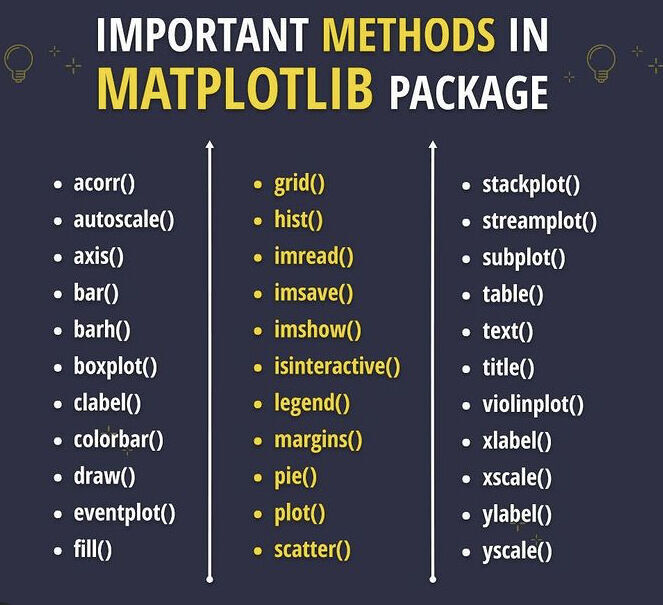
\includegraphics[scale=.9]{../img/python/matplotlib.jpeg}
    \caption{Matplotlib}
    \label{img:matplotlib}
\end{figure}


\underline{Seaborn}~\footnote{https://seaborn.pydata.org/}

\begin{figure}[!htp]
    \centering
    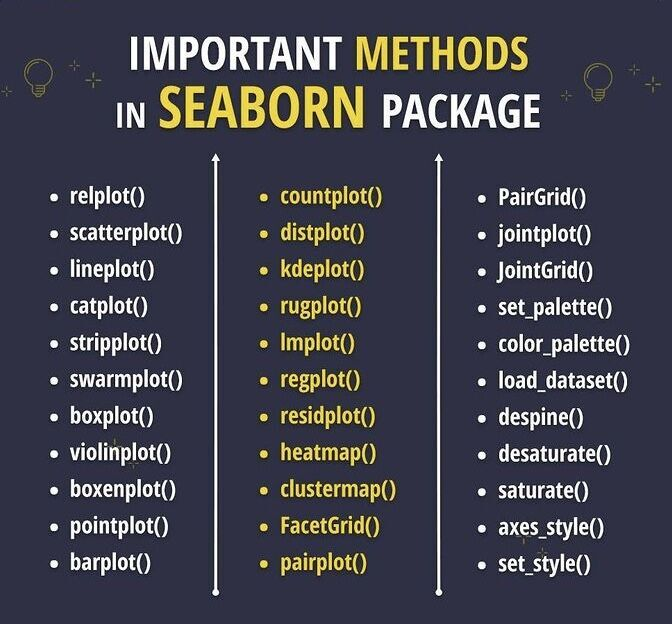
\includegraphics[scale=.5]{../img/python/seaborn.jpeg}
    \caption{Seaborn}
    \label{img:seaborn}
\end{figure}

\underline{Plotly Dash}~\footnote{https://plotly.com/} é uma ferramenta que atual em diversas linguagens de modo interativo em um servidor local.
Além disso, utiliza Flask~\footnote{https://flask.palletsprojects.com}, React.js~\footnote{https://reactjs.org} e CSS para definir o design dos gráficos.
Exemplo do funcionamento do Plotly Dash é ministrado pelo Eduardo Mendes~\footnote{https://www.youtube.com/watch?v=fKgPXUUsg1M}


\underline{Moving Pandas}~\footnote{https://anitagraser.github.io/movingpandas/}


\underline{Geo Pandas}~\footnote{https://geopandas.org/}